\documentclass[11pt, a4paper]{article}
\usepackage[nochapters]{classicthesis}                              % template
\usepackage[margin=42mm]{geometry}                                  % margins
\usepackage[utf8]{inputenc}                                         % allow utf-8 input
\usepackage[T1]{fontenc}                                            % use 8-bit T1 fonts
\usepackage{graphicx}                                               % images
\usepackage{url}                                                    % URL typesetting
\usepackage{booktabs}                                               % good-looking tables
\usepackage{multirow}                                               % for tables
\usepackage{amsfonts}                                               % blackboard math symbols
\usepackage{amsmath}                                                % math ops
\usepackage{nicefrac}                                               % compact 1/2, etc.
\usepackage{microtype}                                              % microtypography
\usepackage{float} %to force figures to appear at a specific location
\usepackage{subcaption}
\usepackage{tabularx}

\definecolor{darkblue}{rgb}{0, 0, 0.5}                              % define link color
\hypersetup{colorlinks=true,citecolor=darkblue,                     % set link color
            linkcolor=darkblue, urlcolor=darkblue}

% Your packages here
% \usepackage{...}                                                  % some info, maybe

% !!! PLEASE CHANGE THESE VARIABLES TO MATCH YOUR INFORMATION !!!

\def\thesistitle{The Main Title of the Thesis}                      % title
\def\subtitle{The Subtitle of the Thesis If It Has One}             % subtitle
    % ^if there is no subtitle, replace by \def\subtitle{}  
\def\yourname{Your Name}                                                                       % ^first and last nam
 \def\yourprogramme{Cognitive Science \& Artificial Intelligence}    % uncomment this
\def\yourstudentnumber{2066623}                                      % ANR (or u-number)
\def\finalmonth{January}
\def\finalyear{2000}
\def\supervisor{dr. Phillip Brown}
\def\committee{dr. Silvia-Laura Pintea}
\def\acknowledgments{Some room for acknowledgements.}
\def\wordcount{your word count should be here, ex 12000}
% METADATA

\hypersetup{pdfauthor   = \yourname,
            pdftitle    = \thesistitle\ \subtitle,
            pdfsubject  = \yourprogramme\ Master Thesis
}

% CHOOSE EITHER OF -----------------------------------------
% IEEE STYLE:

% \usepackage[square,numbers]{natbib}                               % bracket-style refs
% \usepackage{natbib}                                               % OR: parenthesized refs
% \bibliographystyle{IEEEtranN}

% OR -------------------

\usepackage[natbibapa]{apacite}                                     % only parentheses
\bibliographystyle{apacite}                                         % 'cause APA

% !!! ------------------------------------------------------ !!!

\begin{document}
\input{frontmatter.tex}  % don't remove this :)

% --- start writing below:

\begin{abstract}
This is where the abstract goes. Don't forget to change the variables in \texttt{main.tex} to change all general placeholders shown in this document. The \texttt{frontmatter.tex} file should be left alone. The abstract should summarize in 150-250 words the contents of the thesis, mentioning: 1) the research goal, 2) the methods employed, 3) data collected or dataset/s used, 4) the main findings.
\end{abstract}

\section{Data Source, Ethics, Code, and Technology statement}
Checklist for creating a Data Source, Ethics, Code, and Technology (DSECT) statement:
Please provide answers to all below questions for transparency purposes when writing your ethical statement. There is no one-fits-all solution to ethical statements, and they heavily
depend on the nature of the study. After the questions below, an example DSECT statement is provided. 
\begin{itemize}
    \item[•] {Data Source}
    \begin{itemize}
        \item[o] {Who is the owner of the data?}
        \item[o] {Does the thesis project involve collecting data from human participants or animals?}
        \item[o] {Does the owner of the data give consent?}
        \item[o] {How and through what channel is the data acquired?}
    \end{itemize}
    \item[•] {Figures}
    \begin{itemize}
        \item[o] {Did you create all the images and figures?}
        \item[o] {Do you have consent for the images that you did not generate?}
    \end{itemize}
    \item[•] {Code}
    \begin{itemize}
        \item[o] {Did you use parts of the code from another study/someone else?}
        \item[o] {Did you list, including version number, all libraries and frameworks used?}
    \end{itemize}
    \item[•] {Technology}
    \begin{itemize}
        \item[o] {Did you use any tools or services to paraphrase the given text (for example a thesaurus or the Academic Phrasebank)? Please name them.}
        \item[o] {Did you use any tools or services to check spelling or grammar? Please name them.}
        \item[o] {Did you use any tools or service to typeset the given text? Please name them.}
        \item[o] {Did you use any reference management software other than the latex template? If so, please name it.}
        \item[o] {The following \textbf{statement should be included}: During the preparation of this work, the author used [NAME TOOL / SERVICE] in order to [REASON]. After using this tool/service, the author reviewed and edited the content as needed and takes full responsibility for the content of the thesis.}
    \end{itemize}
\end{itemize}


A DSECT Statement can be generated by answering the questions listed above and excluding the questions when not applicable.\

\subsection{Source/Code/Ethics/Technology Statement Example} \label{subs:DESCT}
Data Source: 
The (DATA) has been acquired from the (DATA SOURCE) through an online request. The obtained data is anonymised. Work on this thesis did not involve collecting data from human participants or animals. The original owner of the data and code used in this thesis retains ownership of the data and code during and after the completion of this thesis. However, the institution was informed about the use of this data for this thesis and potential research publications.
All the figures but Figure A and B belong to the author. To use Figure A and Figure B, the author received written permission via an email from FIGURE OWNER (AFFILIATION). The thesis code can be accessed through the GitHub repository following the link [CODE LINK].
Part of the CODE has been adapted by the author from (SOURCE, licensed under a CC0 BY 4.0). The reused/adapted code fragments are clearly indicated in the notebook. In terms of writing, the author used assistance with the language of the paper. A generative language
model (MODEL NAME + SOURCE) was used to improve the author's original content, for paraphrasing, spell checking and grammar. No other typesetting tools or services were used.


\section{Introduction} \label{sec:introduction}
In the aviation industry, pilot training plays a vital role and is directly linked to both flight safety and the effective execution of flight operations \citep{Yang2021}. However, the current training framework is largely instructor-led and and may lead to high workload, subjective trainee evaluation, and a lack of real-time feedback on risky behaviors \citep{Yang2021}. Multiple studies have examined the integration of machine learning (ML) techniques with virtual reality (VR) to address these challenges; however, the adoption of ML in pilot training and education remains comparatively underexplored \citep{Caballero et al., 2023}. Machine learning techniques leveraging physiological
signals from trainee pilots incorporate more readily into legacy training equipment \citep{Caballero et al., 2023}; moreover, they enable precise error measurement, replacing labor-intensive
evaluation processes typically performed by human instructors \citep{Barry2025}.

You can refer to chapters like the current Section~\ref{sec:introduction}. If you want to list research questions it's probably best to use \texttt{quote} and/or \texttt{itemize}, like so:

\begin{quote}
\emph{To what extent we define a main research question?}
\end{quote}

\noindent The sub-questions can be listed seperately, as such:

\begin{itemize}
    \item[RQ1] \emph{How does sub question one influence the main RQ?}
    \item[RQ2] \emph{To what degree does sub question add anything?}
\end{itemize}

\noindent Or, format it as you desire (tip: you can nest \texttt{itemize} as well). You can alternate \emph{emph} and \textbf{textbf} however you wish. This should cover most of the things required for the introduction.

\section{Related Work}

Here you provide a synthesis of the existing literature, comparing and drawing parallels across studies to establish the state-of-the-art. Cite relevant theories, models, and recent work. Describe what prior research has found, any contradicting findings or competing approaches. Identify any gaps or limitations in existing research and how your thesis potentially addresses these gaps in terms of methodology, data used, etc.

Copy paste BibTeX code\footnote{Using e.g. the quote icon in GScholar, then BibTeX at the bottom.} and put it in \texttt{references.bib}. After, you can cite some work \citep{mackay2003information} -- using \texttt{\textbackslash citep}. You can refer to the author of e.g. \cite{minsky1961steps} directly like using \texttt{\textbackslash cite} (this does not work when using bracket-citation). If you use bracket-style,\footnote{Find the \texttt{natbib} part in the \texttt{main.tex} \LaTeX{} script.} you might want use \texttt{\textbackslash citeauthor} when citing, like: see \citeauthor{ananny2018seeing} \cite{ananny2018seeing}.  If you want to add pages you can use brackets in \texttt{\textbackslash citep[][p. 5]\{mackay2003information\}}, which looks like: \citep[][p. 5]{mackay2003information}. The first brackets can be used for things like \emph{see}, and \emph{e.g.}. If you want to cite multiple authors, simply comma-separate them (\texttt{\textbackslash citep\{\-minsky\-1961\-steps,\-mackay\-2003\-information\}}) and it will aggregate them automatically \citep{minsky1961steps,mackay2003information}.

\section{Methods}
The following sections describe the dataset, the extraction of physiological and aircraft features in sliding time windows, and the construction of multi‑output targets. They also provide a brief summary of the machine learning model training and the metrics used for evaluation.

\subsection{Dataset}
The CogPilot dataset \citep{Rao2022} was used in this project and is publicly available via PhysioNet \citep{Goldberger2000}. The dataset contains multimodal physiological, task performance, and interaction data collected from 35 participants who each performed flight–landing tasks at various difficulty levels. In a virtual reality environment, each participant followed an Instrument Landing System (ILS) approach and primarily relied on cockpit instrument readings to land an aircraft along a prescribed ideal flight path. Each experimental session consisted of three blocks with four missions per block, resulting in twelve missions per participant, with one difficulty level per mission.

Multiple wearable sensors were used to record seven physiological modalities, with nominal sampling rates ranging from 128 to 1024 Hz \citep{Rao2022}. These modalities comprise electromyography (EMG), accelerometry (ACC), electrodermal activity (EDA), electrocardiography (ECG), respiration (RESP), eye tracking (ETK), and photoplethysmography (PPG). A detailed overview of the functional data derived from each physiological signal is provided in Table 4 in Appendix~A. Mission difficulty was manipulated via four distinct weather conditions \citep{Rao2022}. According to the dataset description, flight performance measures were derived from the simulated aircraft behavior and grouped into three components \citep{Rao2022}. The first two are the localizer and glide slope errors, defined as the angular deviations from the ideal horizontal and vertical landing trajectories \citep{Rao2022}, respectively, each ranging from -3 to 3 degrees. The third component is the absolute deviation from the ideal airspeed, where the raw airspeed error was divided by 10 so that the maximum error is mapped to the same -3 to 3 scale \citep{Rao2022}.

\subsection{Feature Engineering}
Recordings of ECG and RESP were selected as the physiological modalities for feature preprocessing and extraction. Heart rate (HR) derived from ECG can be used as a practical signal for real‑time adaptation of task difficulty to maintain trainees within an optimal workload range \citep{Koerner2025}, and respiratory behavior is a robust marker of cognitive processing, with mentally demanding tasks typically associated with an increased breathing rate (BR) and higher‑frequency ventilation \citep{Grassmann2016}.

The raw ECG signal was first band‑pass filtered between 8 and 20~Hz using a Butterworth filter, as this passband has been shown to be optimal for QRS complex detection with a favorable signal‑to‑noise ratio \citep{Elgendi2010}. R‑peaks were then detected in the cleaned signal using the QRS detection algorithm proposed by \citet{Elgendi2010}. Subsequently, the signal‑quality index (SQI) mechanism from \citet{Zhao2018} was applied to identify low‑quality ECG segments, and HR was computed from the detected R‑peaks only for 25 subjects with ECG recordings classified as having excellent quality.

For the RES signals, an optimized breath detection algorithm developed by \citet{Khodadad2018} was used to preprocess the respiratory traces and to derive breathing rate and respiratory peaks. This method has been shown to outperform conventional algorithms on breath detection in terms of receiver–operating–characteristic performance. Respiratory amplitude was computed as the difference between each respiratory peak and its preceding trough. 

Because ECG and RESP were recorded using the same sensing device, no additional timestamp alignment was required between these two signals. For each subject, difficulty level, and run number, physiological and aircraft features were extracted within a sliding 10~s window that was aligned to the performance timestamps. First, the performance, ECG, RESP, and aircraft data streams were converted from MATLAB time format to seconds and aligned by correcting for the offset between the start times of the performance and physiological recordings, yielding a common time axis for all signals. A 10~s window $(t-10, t]$ was then defined and advanced in 1~s steps along the aligned performance timeline. For each window, the last available performance sample was used to assign the glide slope, localizer, airspeed, and total error as target variables at time $t$.

Within the same 10~s interval, the corresponding segments of the cleaned HR and respiration signals were selected, and the following time‑domain features were computed: the mean, standard deviation, minimum, maximum, and range of HR; the mean and standard deviation of BR; and the mean and standard deviation of respiratory amplitude. In parallel, the mean aircraft elevation trim, aileron trim, and landing‑gear position were computed over the window. Each window thus yielded a single feature vector, comprising physiological and aircraft features, paired with the contemporaneous performance errors, resulting in a second‑by‑second sequence of 10~s summary observations for subsequent modeling.

\subsection{Machine Learning Setup}
All predictive analyses were conducted on subject‑level dataframes constructed from the 10‑s windows described above. For each subject, difficulty level, and run, physiological, aircraft, and performance information were aggregated into a feature matrix and a multi‑output target matrix, where each row represents one time window and the targets correspond to glide slope, localizer, airspeed, and total error. Two feature configurations were considered. In the no‑lag condition, the feature set contained only physiological and aircraft features derived from the current window. In the lag condition, the feature set was augmented with lagged performance measures corresponding to the four target variables at the preceding one and two seconds, thereby enabling the models to exploit very recent performance history.

To quantify generalization, two cross‑validation strategies were implemented that respect the hierarchical and temporal structure of the data. For subject‑level generalization, leave‑one‑subject‑out cross‑validation was applied using the subject identifier as grouping variable, such that all windows from one participant were held out as test data in each fold and the models were trained on the remaining participants. For within‑run temporal generalization, the final 60 s of data in each run of the subjects were excluded from the training–validation set, flagged as temporal test segments, and retained exclusively for final evaluation. On the remaining data , grouped 5‑fold cross‑validation was used, with groups defined as unique subject–run combinations so that all windows from a given run were assigned to the same fold. In both evaluation schemes, hyperparameter tuning was carried out within the respective cross‑validation procedure on the training–validation set only; the selected configuration was then refitted on the full training–validation data before testing.

Three tree‑based regression algorithms were used for model training and evaluation: Random Forest (RF), XGBoost (XGB), and CatBoost (CB). Barry et al. (2025) implemented the same models on this dataset using an ad‑hoc approach to predict performance error; the present study extends this work by systematically examining real‑time forecasting performance across feature configurations (lag vs. no‑lag) and generalization strategies. For each algorithm, a discrete hyperparameter grid was specified to reflect key design choices (e.g., number of trees or boosting iterations, maximum tree depth, and column subsampling rate), and hyperparameter optimization was performed using exhaustive grid search with cross‑validation (GridSearchCV). The negative root mean squared error, averaged across output variables, served as the selection criterion for the best estimator. The explored hyperparameters and their candidate values are summarized in Table 1.

\begin{table}[htbp]
	\caption{Candidate model hyperparameters}
	\label{tab:results}
	\centering
	\small
	\begin{tabular}{lll}
		\toprule                                 	
		Model                        &  Hyperparameter        		&  Values      \\ 
		\midrule
		\multirow{4}{*}{Random Forest}  & Number of Estimators         	& [50, 100, 150] \\
										& Minimum Samples per Split    	& [2, 3, 4] \\
										& Minimum Samples per Leaf     	& [2, 3, 4]   \\
										& Bootstrapping					& [True, False] \\
		\midrule
		\multirow{3}{*}{XGBoost}  		& Number of Estimators          & [10, 100]      \\
										& Maximum Depth   				& [2, 3, 4, 5]    \\
										& Columns Sampled by Tree       & [0.3, 0.4, 0.5]  \\
		\midrule
		\multirow{3}{*}{CatBoost}       & Maximum Depth          		& [2, 3] \\
										& Learning Rate					& [0.01, 0.02, 0.03, 0.05]\\
										& L2 Regularization Coefficient	& [6, 10] \\
		\bottomrule
	\end{tabular}
\end{table}

\subsection{Evaluation Metrics}
Model performance was evaluated using root mean squared error (RMSE), mean absolute error (MAE), and the coefficient of determination $R^2$. RMSE quantifies prediction error in the same units as the target variables and places greater weight on larger errors (Barry, 2025), whereas MAE provides a complementary, more robust measure of typical error magnitude that is less sensitive to outliers. $R^2$ captures the proportion of variance in each target explained by the model and serves as the primary indicator of overall model fit in the Results section. For each cross‑validation setting, the mean and standard deviation of these metrics across folds are reported, along with an overall mean aggregated across targets.

Furthermore, to assess whether the models preserved the relationships between specific error components and overall performance, Pearson correlations between component errors (glideslope, localizer, airspeed) and total error were examined for both true values and model predictions. These correlations were computed across all test samples within each evaluation setting and are reported alongside the primary error metrics.

\subsection{Implementation}
All preprocessing, modeling, and analysis code was implemented in Python using NeuroKit2, pandas, NumPy, and scikit-learn for data handling and the baseline model, XGBoost and Catboost for gradient boosting models, and Matplotlab/seaborn for visualization. Model explainability was examined using SHapley Additive exPlanations (SHAP) to inspect feature contributions for selected outputs. For each final model, SHAP values were computed on a subsample of 1,000 time points, and summary plots as well as local waterfall plots were generated to identify which features most strongly influenced the predicted performance errors.

\section{Results}
This section reports the performance of three tree‑based models for task performance prediction. First, overall subject‑level and temporal generalization performance relative to the Random Forest baseline is summarized; next, error correlations and feature importance are examined.

\subsection{Subject-level Generalization}
In this section, how well the three models generalize to unseen pilots in the subject-level evaluation is presented, first in terms of average performance across subjects and outputs, then in terms of individual error types and per-subject variability.

Table 2 presents the mean MAE, RMSE, and $R^2$ across outputs and subjects for the Random Forest baseline, XGBoost, and CatBoost, with and without lagged features. In the no-lag condition, all models generate negative overall $R^2$ values, indicating performance below a simple mean predictor, with Random Forest showing the worst fit and CatBoost the best of the tree. When lag features are included, overall $R^2$ increases to approximately 0.96 for Random Forest and XGBoost and to 0.97 for CatBoost, accompanied by marked reductions in MAE and RMSE.

Per‑output performance for the best subject‑level model (CatBoost with lag features) is reported in Table 3. For glide slope and localizer errors, $R^2$ values of approximately 0.98 indicate that the model captures most of the between‑subject variance in these errors. Airspeed error is slightly more difficult to predict, with $R^2$ values around 0.96, whereas total error shows somewhat lower but still high explained variance ($R^2$ $\approx$ 0.97). The corresponding Figure 5 in Appendix A shows that predicted values cluster tightly around the identity line for all outputs, confirming that both the direction and the magnitude of subject‑level deviations are reproduced well.

\begin{table}[htbp]
	\caption{Overall subject‑level generalization performance of the models, with and without lagged features.}
	\label{tab:results}
	\centering
	\small
	\begin{tabular}{lccc}
		\toprule                                 	
		Model          	&  Mean MAE      &  Mean RMSE      & Mean $R^2$ \\ 
		\midrule
		Random Forest (no-lag)  	& 0.71  	& 0.97  & -1.21 \\
		Random Forest (lag)         & 0.07 	& 0.12 & 0.96 \\
		\midrule
		XGBoost (no-lag)  	& 0.69  	& 0.91  & -0.83\\
		XGBoost (lag)         & 0.07 	& 0.12 & 0.96 \\
		\midrule
		CatBoost (no-lag)  	& 0.67  	& 0.89 & -0.67 \\
		CatBoost (lag)         & 0.05 	& 0.10 & 0.97\\ 
		\bottomrule
	\end{tabular}
\end{table}

Figure 2 compares the RMSE of total error per subject for the Random Forest and CatBoost models with lag features. For all subjects, CatBoost generally achieves slightly lower RMSE than Random Forest. The most noticeable gains occur for subjects exhibiting relatively high baseline errors. For most pilots, changing the model architecture offers only limited additional benefit beyond the inclusion of lagged features. For glide slope and localizer errors, the mean RMSEs in the subject‑level setting are low (approximately 0.07–0.08), but the corresponding standard deviations are relatively large (approximately 0.05–0.09). This pattern reflects substantial variability across pilots: some subjects show very small errors, whereas others retain noticeably higher prediction errors, indicating that generalization quality is not uniform across individuals.

\begin{table}[htbp]
	\caption{Per-output performance for CatBoost with lagged features (subject level generalization).}
	\label{tab:results}
	\centering
	\small
	\begin{tabular}{lccc}
		\toprule                                 	
		Output          	& MAE      & RMSE      & $R^2$ \\ 
		\midrule
		Glide slope 	& 0.03\textpm0.01  	& 0.07\textpm0.05  & 0.98\textpm0.03\\
		\midrule
		Localizer    & 0.03\textpm0.02  	& 0.08\textpm0.09  & 0.98\textpm0.02\\
		\midrule
		Airspeed	& 0.07\textpm0.01  	& 0.12\textpm0.02  & 0.96\textpm0.04\\
		\midrule
		Total        & 0.08\textpm0.03  	& 0.14\textpm0.04  & 0.97\textpm0.03\\
		\bottomrule
	\end{tabular}
\end{table}

\begin{figure}[htbp]
	\centering
	
\includegraphics[width=\textwidth]{rmse_total_error_RF_vs_Cat_per_subject.png}
	\caption{Comparison of total‑error RMSE per subject for Random Forest and CatBoost models with lagged features} 
	\label{fig:probs}
\end{figure}

\subsection{Temporal Generalization}
Table 4 presents temporal generalization performance, averaged across outputs for the three models, with and without lag features. In the no-lag condition, all models achieve modest predictive accuracy, with overall $R^2$ values around 0.20, and RMSE close to 1.17. Including lag features has a substantial improvement across models: overall $R^2$ increases to approximately 0.97 for Random Forest and to about 0.98 for XGBoost and CatBoost, while MAE and RMSE decrease by about a factor of ten. Among the three models, CatBoost with lag features attains the lowest overall errors (MAE $\approx$ 0.07, RMSE $\approx$ 0.16).

\begin{table}[htbp]
	\caption{Overall temporal generalization performance of the models, with and without lag features}
	\label{tab:results}
	\centering
	\small
	\begin{tabular}{lccc}
		\toprule                                 	
		Model          	&  Mean MAE      &  Mean RMSE      & Mean $R^2$ \\ 
		\midrule
		Random Forest (no-lag)  	& 0.68  	& 1.13  & 0.20 \\
		Random Forest (lag)         & 0.09 	& 0.19 & 0.97 \\
		\midrule
		XGBoost (no-lag)  	& 0.75  	& 1.17  & 0.18\\
		XGBoost (lag)         & 0.09	& 0.18 & 0.98 \\
		\midrule
		CatBoost (no-lag)  	& 0.73  	& 1.15 & 0.20 \\
		CatBoost (lag)         & 0.07 	& 0.16 & 0.98\\ 
		\bottomrule
	\end{tabular}
\end{table}

Temporal performance per output for the three models in the lag condition is detailed in Table 5. For glide slope and airspeed errors, all models achieve high explained variance, with $R^2$ above 0.97 and RMSE below 0.20, indicating accurate prediction of future deviations within runs. Localizer error is slightly more difficult to predict, with $R^2$ of approximately 0.96, although absolute errors remain small. CatBoost performs best overall, showing higher $R^2$ and lower MAE and RMSE than the other two models.

\begin{table}[htbp]
	\caption{Temporal performance per output of three models in the lag condition}
	\label{tab:results}
	\centering
	\small
	\begin{tabular}{lcccc}
		\toprule
		Model / Metrics  & Glide slope & Localizer & Airspeed & Total Error \\
		\midrule
		RF MAE           & 0.09 & 0.07 & 0.09 & 0.12 \\
		RF RMSE          & 0.20 & 0.21 & 0.15 & 0.21 \\
		RF $R^2$         & 0.98 & 0.95 & 0.98 & 0.99 \\
		\midrule
		XGB MAE          & 0.08 & 0.06 & 0.07 & 0.13 \\
		XGB RMSE         & 0.18 & 0.19 & 0.13 & 0.23 \\
		XGB $R^2$        & 0.98 & 0.96 & 0.98 & 0.99 \\
		\midrule
		CB MAE          & 0.06 & 0.05 & 0.06 & 0.10 \\
		CB RMSE         & 0.15 & 0.18 & 0.11 & 0.19 \\
		CB $R^2$        & 0.99 & 0.96 & 0.99 & 0.99 \\
		\bottomrule
	\end{tabular}
\end{table}

The comparison between no‑lag and lag conditions in Figure 3 highlights the role of short‑term history in temporal prediction. For example, the RMSE of CatBoost for total error decreases from approximately 1.59 to 0.19 when lagged features are added, and the corresponding $R^2$ increases from 0.34 to 0.99. Similar improvements are observed for Random Forest and XGBoost. These results suggest that including preceding error is essential for accurate forecasting of near‑future task performance.

\begin{figure}[htbp]
	\centering
	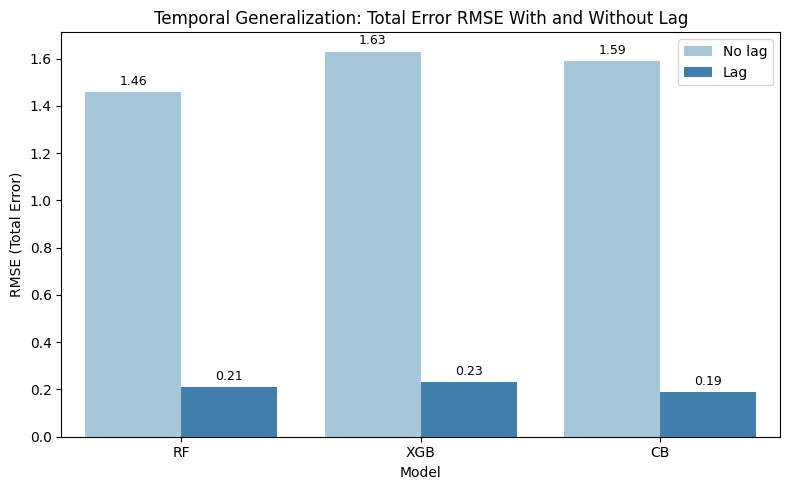
\includegraphics[width=\textwidth]{temporal total-error RMSE .png}
	\caption{Comparison of total‑error RMSE in temporal generalization for three models with and without lagged features} 
	\label{fig:probs}
\end{figure}

Comparing Tables 2 and 4 shows that generalization to unseen pilots is slightly more difficult than temporal prediction within runs. In the lag condition, all models achieve higher $R^2$ for temporal prediction than for subject‑level prediction. This pattern suggests that individual pilots exhibit consistent short‑term dynamics that can be exploited to anticipate upcoming deviations, whereas cross‑subject variability remains more challenging to model.

\subsection{Error Correlations and Feature Importance}
Table 6 reports Pearson correlations between true component errors and true total error. The true data show only weak associations between individual component errors and total error, indicating that overall error combines several largely distinct parts rather than being dominated by a single component. Correlations between predicted individual errors and true total error are presented in Table 9 in Appendix A. In the subject-level and temporal no-lag conditions, these correlations are small and do not match the corresponding correlations observed in the true data, and predicted total error correlates only moderately with the true values, with Pearson's r ranging from approximately 0.22 to 0.70 depending on model and generalization setting.

\begin{table}[htbp]
	\caption{Pearson correlations between true component errors and true total error}
	\label{tab:results}
	\centering
	\small
	\begin{tabular}{lcc}
		\toprule
		& \multicolumn{2}{c}{Pearson Correlation} \\
		\cmidrule{2-3}            	
		Component Error      & Subject-level & Temporal   \\ 
		\midrule
		Glide Slope  	& 0.09 & 0.10\\
		\midrule
		Localizer        & -0.20 & -0.10\\
		\midrule
		Airspeed  	& 0.22 & 0.20\\
		\bottomrule
	\end{tabular}
\end{table}

In contrast, in the lag conditions, all three models match the observed correlation pattern more closely. For both subject-level and temporal generalization, predicted component errors exhibit correlations with total error that closely resemble the true correlations. The correlation between predicted and true total error reaches 0.99 across models. These results indicate that the models achieve accurate predictions of total error and, at the same time, reproduce the observed relationships between the individual error components and overall approach performance. Figure 4 and 5 illustrates these relationships for the CatBoost model under the lag condition, showing that the regression lines for the predicted component errors closely follow those of the true errors across the range of total error.

\begin{figure}[htbp]
	\centering
	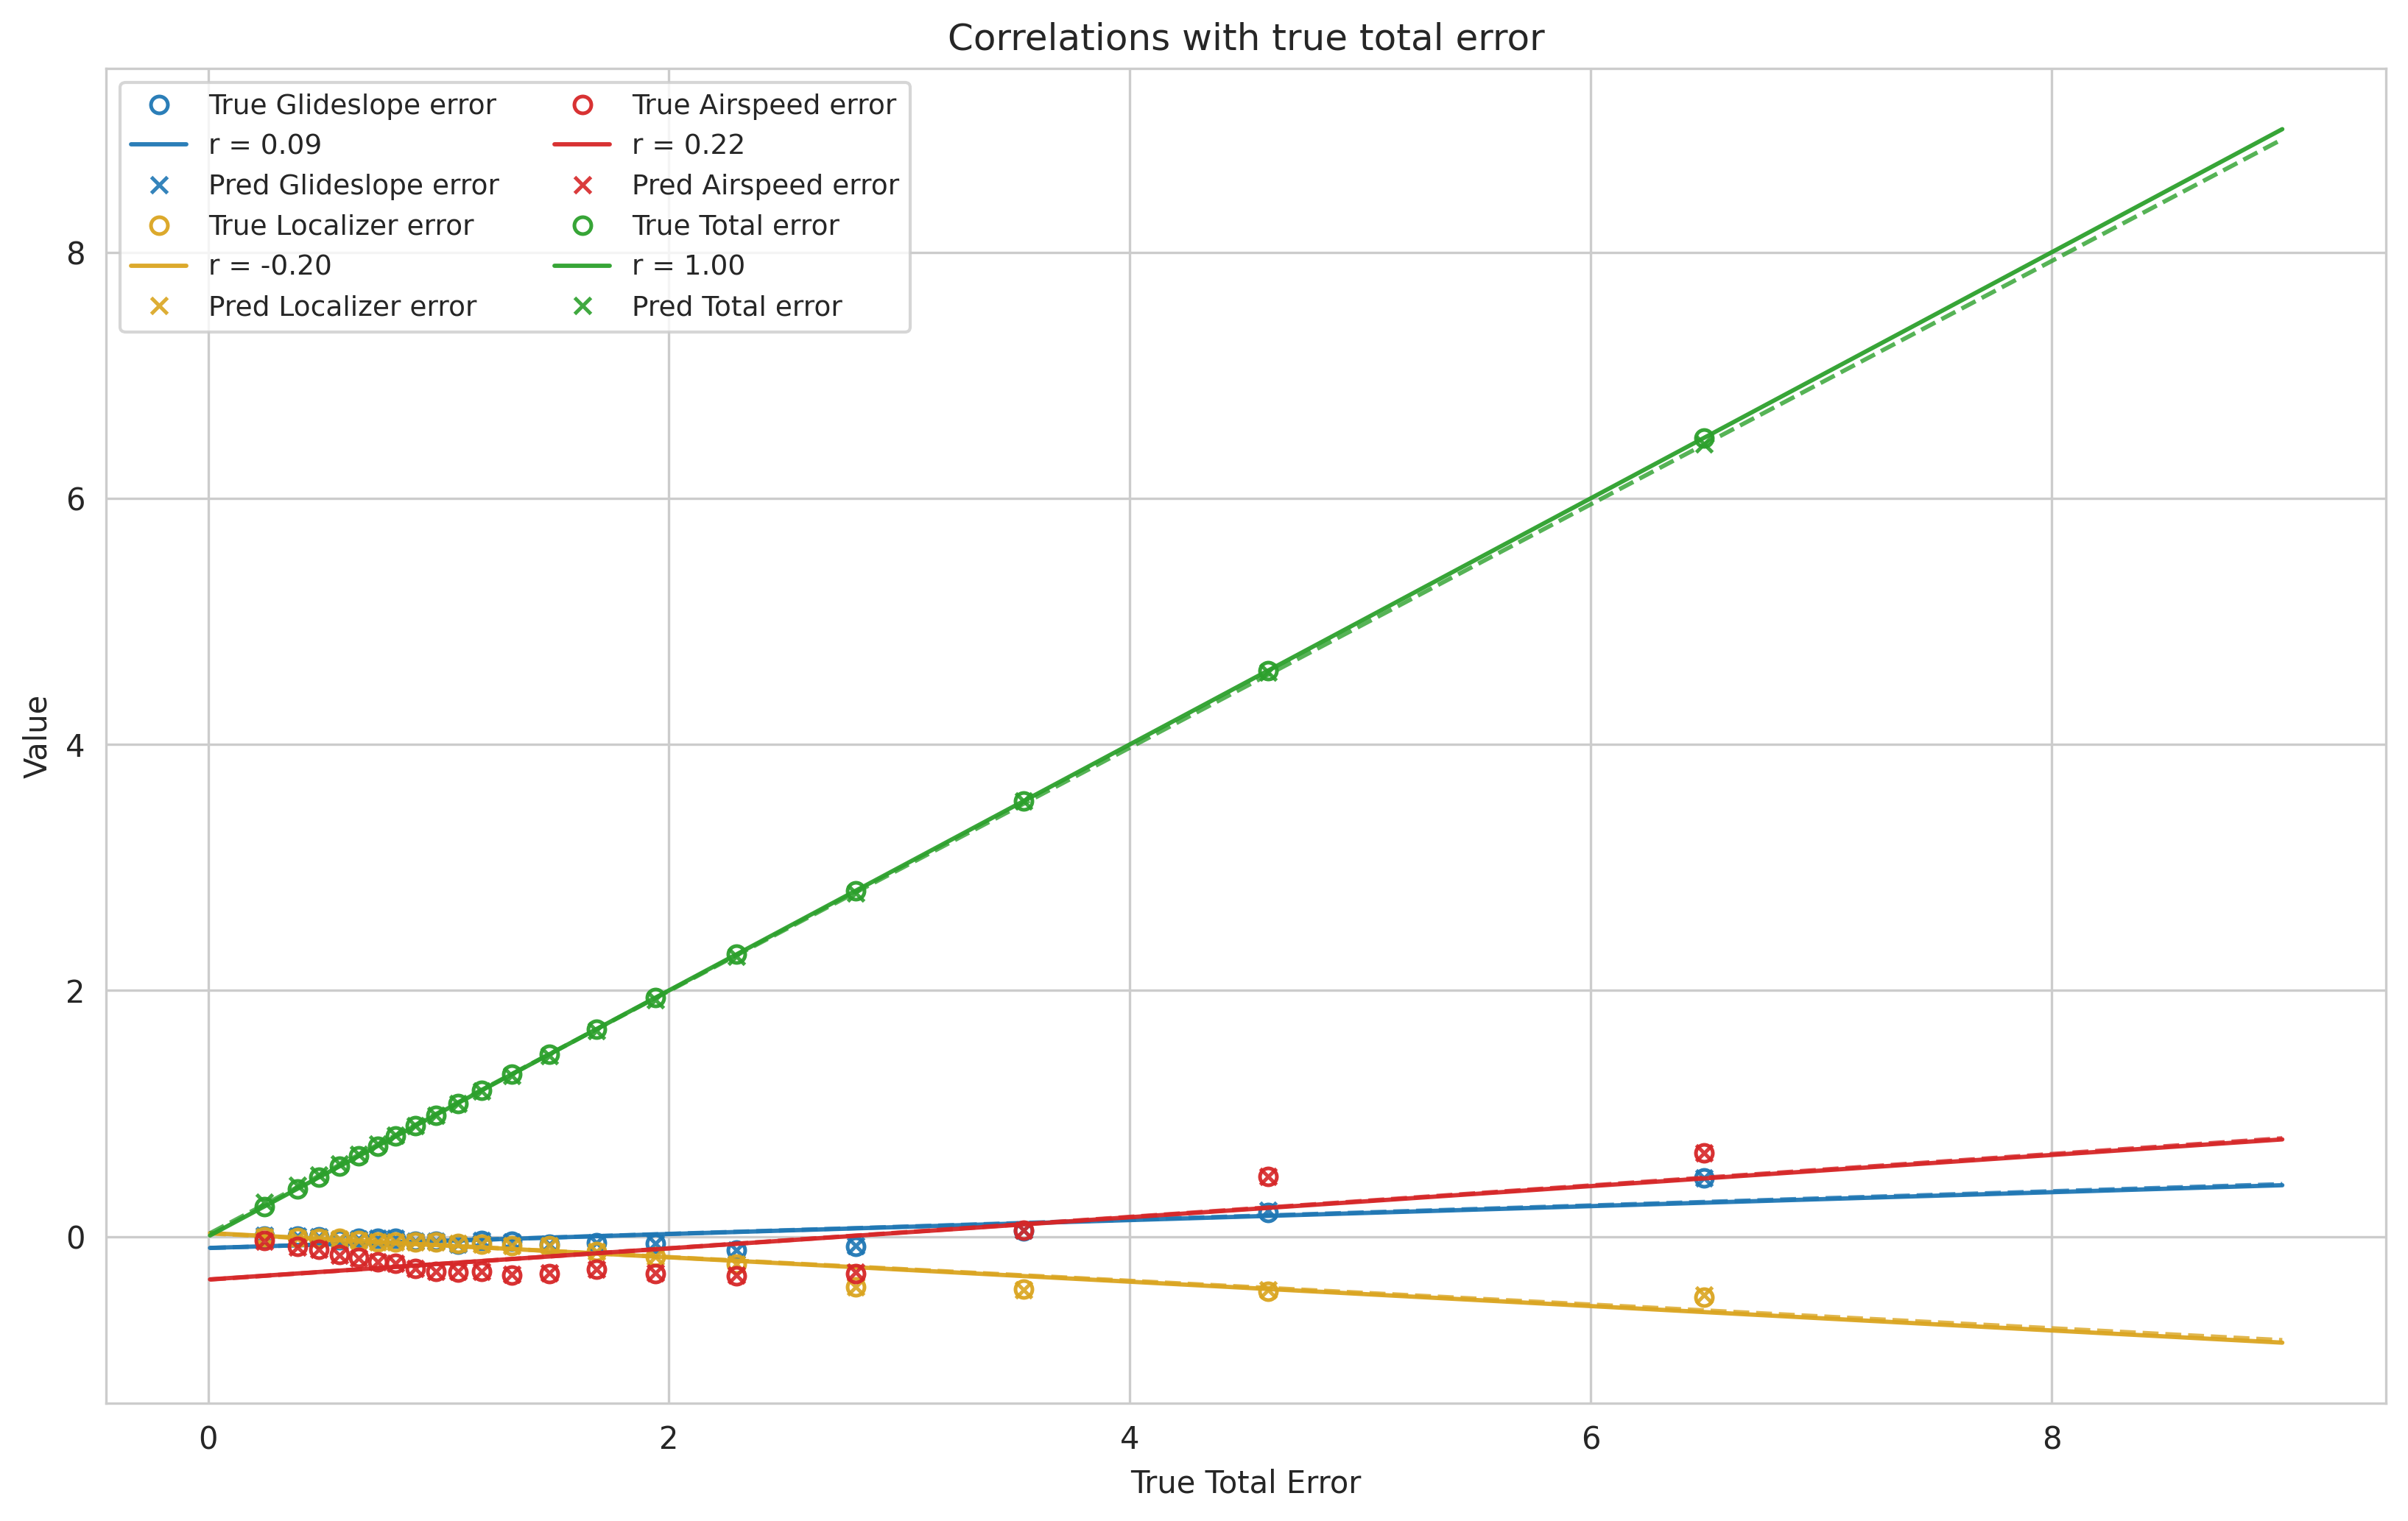
\includegraphics[width=\textwidth]{corr_vs_true_total_error_subject_lag.png}
	\caption{Correlations between component errors and the true total error for CatBoost (subject-level generalization with lag features) }
	\label{fig:corr-sub-lag}
\end{figure}
\begin{figure}[htbp]
	\centering
	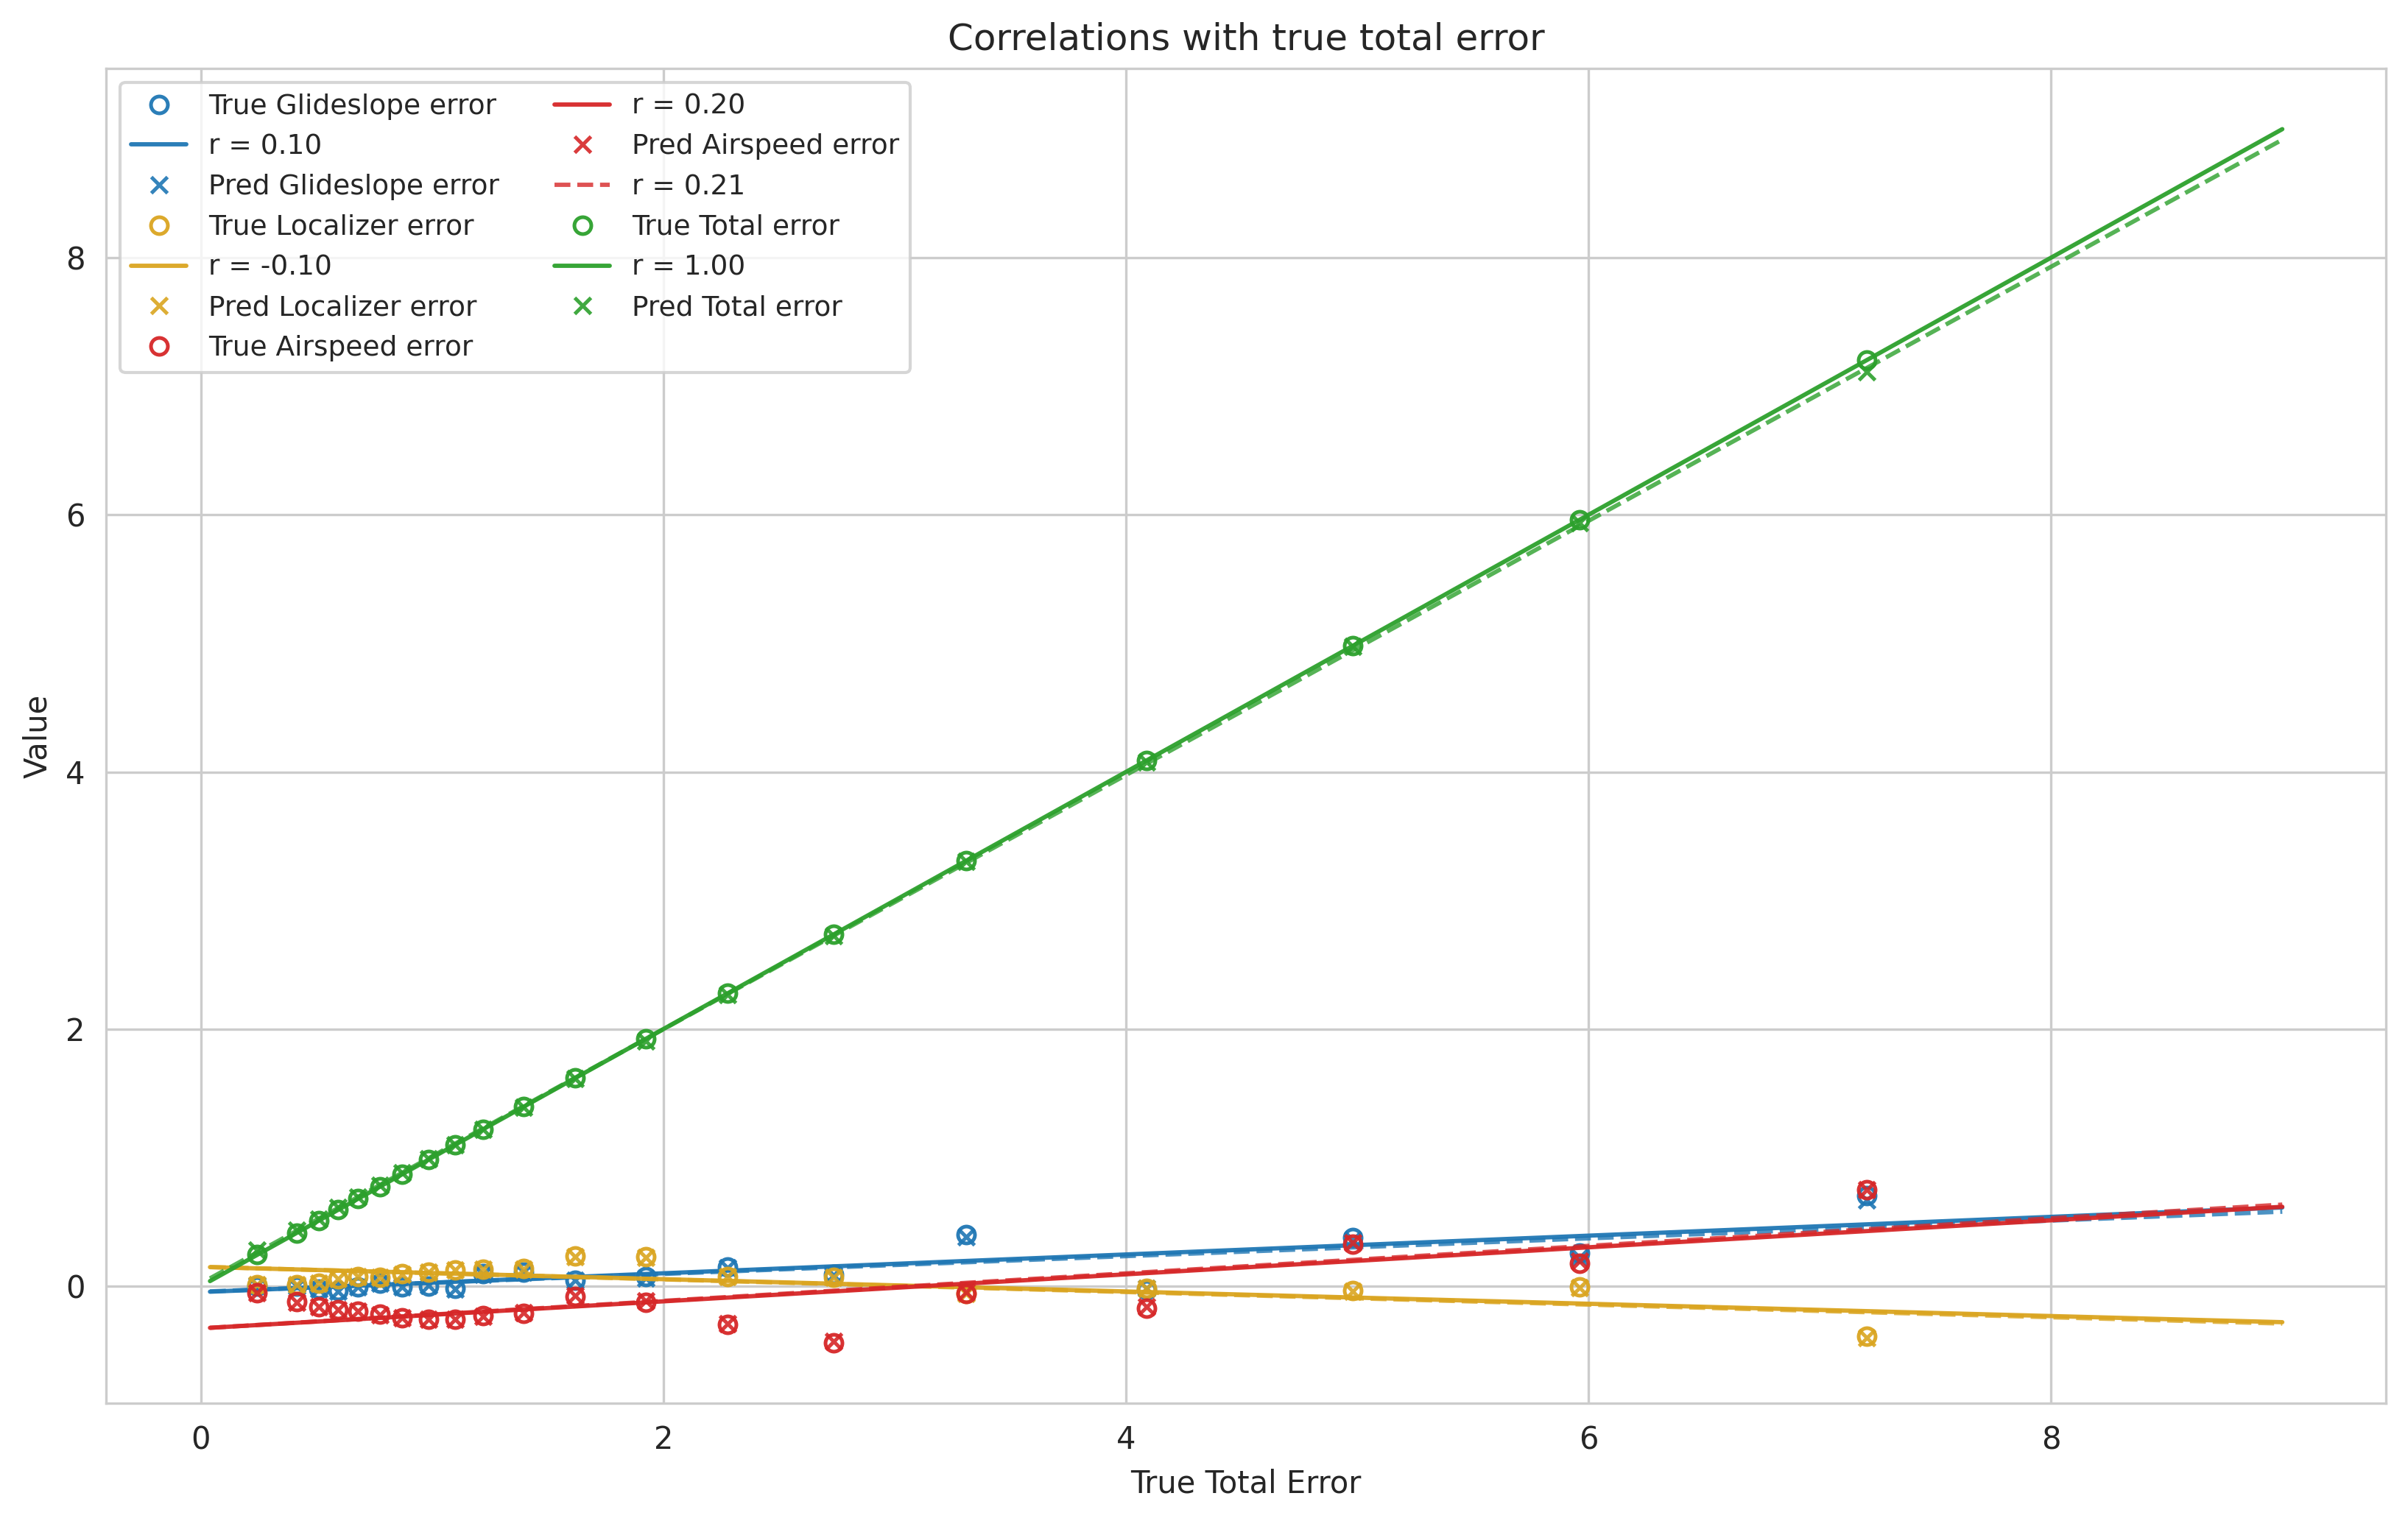
\includegraphics[width=\textwidth]{corr_vs_true_total_error_temporal_lag.png}
	\caption{Correlations between component errors and the true total error for CatBoost (temporal generalization with lag features)}
	\label{fig:corr-temp-lag}
\end{figure}

Feature importance analyses for the models in the no‑lag condition, as shown in Table 11 and 12 in Appendix A, indicate that elevation, aileron, and physiological variables related to heart rate and respiration are the most influential predictors of the performance variables. For example, Random Forest and XGBoost assign the highest importance to mean elevation trim and mean aileron trim, followed by heart‑rate range and breathing‑related features.

\begin{table}[htbp]
	\caption{Feature importance for subject-level generalization (lag condition).
		Only the most influential lag features are shown.}
	\label{tab:results}
	\centering
	\small
	\begin{tabular}{lccc}
		\toprule
		Feature & Random Forest & XGBoost & CatBoost \\
		\midrule
		Total Error (lag1)          & 0.5211 & 0.0193 & 80.3380 \\
		Total Error (lag2)          & 0.0006 & 0.1728 & 19.1385 \\
		Airspeed Error (lag2)    & 0.0010 & 0.0537 &  0.1709 \\
		Airspeed Error (lag1)    & 0.1424 & 0.1776 &  0.1596 \\
		Glide Slope Error (lag1) & 0.1989 & 0.2410 &  0.0513 \\
		Glide Slope Error (lag2) & 0.0022 & 0.0560 &  0.0509 \\
		Localizer Error (lag1)   & 0.1259 & 0.0873 &  0.0258 \\
		Localizer Error (lag2)   & 0.0045 & 0.1616 &  0.0117 \\
		\bottomrule
	\end{tabular}
\end{table}

When lagged features are included, the importance pattern changes substantially, as presented in Table 7 and 8. In all three models, lagged performance variables become the primary predictors. The first lag of total error receives the highest importance, followed by the first lags of glide slope, airspeed, and localizer errors. The second lags and sensor features have much smaller importance scores. This pattern indicates that recent performance history is the strongest predictor of future errors, while elevation trim, and physiological variables have additional but relatively modest effects.

\begin{table}[htbp]
	\caption{Feature importance for temporal generalization (lag condition).
		Only the most influential lag features are shown.}
	\label{tab:results}
	\centering
	\small
	\begin{tabular}{lccc}
		\toprule
		Feature & Random Forest & XGBoost & CatBoost \\
		\midrule
		Total Error (lag1)       & 0.5235 & 0.0215 & 89.8342 \\
		Total Error (lag2)       & 0.0008 & 0.1533 &  9.6466 \\
		Airspeed Error (lag2)    & 0.0011 & 0.0381 &  0.1909 \\
		Airspeed Error (lag1)    & 0.1523 & 0.1851 &  0.1743 \\
		Localizer Error (lag1)   & 0.1261 & 0.0986 &  0.0311 \\
		Glide Slope Error (lag2) & 0.0193 & 0.0674 &  0.0238 \\
		Glide Slope Error (lag1) & 0.1679 & 0.2328 &  0.0220 \\
		Localizer Error (lag2)   & 0.0045 & 0.1668 &  0.0121 \\
		\bottomrule
	\end{tabular}
\end{table}

SHAP analysis for the CatBoost model in the temporal generalization setting with lag features confirms the feature‑importance findings. The SHAP summary plot (Figure 6 in Appendix A) shows that lagged total error from the preceding one second has the largest impact on the predicted total error, followed by lagged total error from the previous two seconds and the lagged airspeed, localizer, and glideslope errors, which is consistent with the dominance of lagged performance variables in the importance rankings. High values of the lagged total error are associated with positive SHAP values, indicating increased predicted total error, whereas low values of this lagged error yield negative SHAP values and thus reduce the prediction. Physiological features such as HR range and mean BR exhibit much smaller SHAP magnitudes, indicating that these variables play only a minor role compared to lagged performance errors in the CatBoost model.

\section{Discussion}


\section{Conclusion}


\bibliography{references}

\appendix
\section*{Appendix A} \label{app:a}

\begin{table}[htbp]
	\caption{Multimodal physiological data}
	\label{tab:results}
	\centering
	\small
	\begin{tabular}{lll}
		\toprule                                 	
		Variable Name                   &  Unit        		&  Description     \\ 
		\midrule
		EMG Wrist Flexor  				& mV         	& EMG of wrist flexor muscles\\
		\midrule
		EMG Wrist Extensor				& mV          & EMG of wrist extensor muscles  \\
		\midrule  			
		PPG Finger   				& mV    & Optical signal at tip of the middle finger \\
		\midrule
		EDA Hand L    				& KOhms          		& EDA measured on the left hand \\
		\midrule
		ECG Projection LL-RA     & mV          		& ECG Signal: LL-RA projection \\
		\midrule
		ECG Projection LA-RA     & mV          		& ECG Signal: LA-RA projection \\
		\midrule
		ECG Projection VX-RL     & mV          		& ECG Signal: VX-RL projection \\
		\midrule
		Respiration Trace     	& mV          		& Respiration Trace \\
		\midrule
		Accelerometry Forearm x/y/z    & \text{m/s\textsuperscript{2}}  & Accelerometry of the right forearm\\
		\midrule
		Accelerometry Torso x/y/z    & \text{m/s\textsuperscript{2}}  & Accelerometry of the torso\\
		\midrule
		Gaze Origin L/R x/y/z		& mm		& Origin point of the gaze ray from each eye \\
		\midrule
		Gaze Direction L/R x/y/z	& mm		& The normalized gaze direction of each eye \\
		\midrule
		Eye Openness L/R  			& - 		& A value representing how open each eye is\\
		\midrule
		Pupil Position L/R x/y/z	& -			& Normalized position of each pupil in sensor area\\
		\midrule
		Pupil Diameter L/R 			& mm		& Diameter of each pupil\\
		\bottomrule	
	\end{tabular}
\end{table}

\begin{figure}[htbp]
	\centering
	\begin{subfigure}{0.48\textwidth}
		\centering
		
\includegraphics[width=\linewidth]{scatter_true_vs_pred_glideslope_error_deg_lag.png}
		\caption{Glide slope}
		\label{fig:sub-glide}
	\end{subfigure}
	\begin{subfigure}{0.48\textwidth}
		\centering
		
\includegraphics[width=\linewidth]{scatter_true_vs_pred_localizer_error_deg_lag.png}
		\caption{Localizer}
		\label{fig:sub-local}
	\end{subfigure}
	\begin{subfigure}{0.48\textwidth}
		\centering
		
\includegraphics[width=\linewidth]{scatter_true_vs_pred_airspeed_error_kts_lag.png}
		\caption{Airspeed}
		\label{fig:sub-air}
	\end{subfigure}
	\begin{subfigure}{0.48\textwidth}
		\centering
		
\includegraphics[width=\linewidth]{scatter_true_vs_pred_total_error_lag.png}
		\caption{Total error}
		\label{fig:sub-total}
	\end{subfigure}
	\caption{True–versus–predicted errors for the best subject-level model.}
	\label{fig:scatter-all}
\end{figure}

\begin{table}[htbp]
	\caption{Pearson correlations between predicted individual errors and true total error}
	\label{tab:results}
	\centering
	\small
	\begin{tabular}{llcc}
		\toprule
		                      &        & \multicolumn{2}{c}{Pearson Correlation} \\
		                      			\cmidrule{3-4}  	
		Individual Error      & Model  & Subject-level & Temporal  \\ 
		\midrule
		\multirow{6}{*}{Glide Slope}  	& RF (no-lag) 	& -0.07	 & 0.08\\
										& RF (lag) 		&  0.09	 & 0.09\\
										& XGB (no-lag) 	& -0.07   & 0.16 \\
										& XGB (lag) 	&  0.09 & 0.10\\
										& CB (no-lag) 	&  -0.10 & 0.16\\
										& CB (lag) 		&  0.09 & 0.10\\
		\midrule
		\multirow{6}{*}{Localizer}      & RF (no-lag) 	&  0.04 & 0.01\\
										& RF (lag) 		& -0.20 & -0.11\\
										& XGB (no-lag) 	&  0.04 & -0.14\\
										& XGB (lag) 	& -0.20 & -0.11\\
										& CB (no-lag) 	& -0.01 & -0.08\\
										& CB (lag) 		&  -0.20 & -0.10\\
		\midrule
		\multirow{6}{*}{Airspeed}  	& RF (no-lag) 	&  0.11 & 0.17\\
									& RF (lag) 		&  0.23 & 0.22\\
									& XGB (no-lag) 	&  0.04 & 0.17\\
									& XGB (lag) 	&  0.22 & 0.21\\
									& CB (no-lag) 	&  0.05 & 0.18\\
									& CB (lag) 		&  0.22 & 0.21\\
		\midrule
		\multirow{6}{*}{Total Error}	& RF (no-lag) 	&  0.28 & 0.70\\
										& RF (lag) 		&  0.99 & 0.99\\
										& XGB (no-lag) 	&  0.24 & 0.61\\
										& XGB (lag) 	&  0.99 & 0.99\\
										& CB (no-lag) 	&  0.22 & 0.64\\
										& CB (lag) 		&  0.99 & 0.99\\
		\bottomrule
	\end{tabular}
\end{table}

\begin{table}[htbp]
	\centering
	\caption{Feature importance for subject-level generalisation without lag
		features. Only the most influential non-lag features are shown; importance
		scores are the model-specific values reported by each algorithm.}
	\label{tab:featimp_subject_nolag}
	\begin{tabular}{lccc}
		\toprule
		Feature & Random Forest & XGBoost & CatBoost \\
		\midrule
		Mean Elevation       & 0.2474 & 0.2219 & 33.7163 \\
		HR Range            & 0.0937 & 0.0618 & 18.2773 \\
		Mean Aileron        & 0.1269 & 0.1382 & 12.4337 \\
		Difficulty Level    & 0.0531 & 0.1336 & 10.6098 \\
		Mean HR             & 0.0655 & 0.0355 &  4.6005 \\
		Mean BR             & 0.0749 & 0.0501 &  4.4261 \\
		SD BR              & 0.0536 & 0.0461 &  3.8130 \\
		Max HR              & 0.0586 & 0.1167 &  5.3498 \\
		Min HR              & 0.0780 & 0.0515 &  1.2061 \\
		SD HR             & 0.0350 & 0.0664 &  0.4180 \\
		Mean RESP Amp       & 0.0711 & 0.0518 &  5.1496 \\
		SD RESP Amp        & 0.0422 & 0.0264 &  0.0000 \\
		\bottomrule
	\end{tabular}
\end{table}

\begin{table}[htbp]
	\centering
	\caption{Feature importance for temporal generalization without lag features.
		Only the most influential non-lag features are shown; importance scores are
		the model-specific values reported by each algorithm.}
	\label{tab:featimp_temporal_nolag}
	\begin{tabular}{lccc}
		\toprule
		Feature & Random Forest & XGBoost & CatBoost \\
		\midrule
		Mean Elevation      & 0.2483 & 0.1537 & 30.0652 \\
		HR Range            & 0.0888 & 0.0656 & 11.6198 \\
		Mean Aileron         & 0.1305 & 0.1117 & 14.9291 \\
		Difficulty Level     & 0.0557 & 0.1356 &  9.5925 \\
		Mean HR             & 0.0623 & 0.0590 &  7.2717 \\
		Mean BR             & 0.0749 & 0.0504 &  6.8984 \\
		SD BR              & 0.0550 & 0.0484 &  4.0880 \\
		Max HR              & 0.0613 & 0.0998 &  5.1017 \\
		Min HR              & 0.0724 & 0.0507 &  3.4167 \\
		SD HR             & 0.0364 & 0.1460 &  0.6144 \\
		Mean RESP Amp       & 0.0735 & 0.0461 &  6.2590 \\
		SD RESP Amp        & 0.0409 & 0.0329 &  0.1434 \\
		\bottomrule
	\end{tabular}
\end{table}

\begin{figure}[htbp]
	\centering
	
\includegraphics[width=\textwidth]{shap_summary_total_error_lag.png}
	\caption{SHAP summary plot for CatBoost (temporal generalization with lag features)} 
	\label{fig:shap-catboost-temp-lag}
\end{figure}

If you have nothing to append: remove this. You can do a page referral for these, like: Appendix A (page~\pageref{app:a}).



\section*{Appendix B}

And this!
\end{document}